\chapter{
  The LHC and CMS Experiment
 }\label{ch_cms}

The physics analysis is carried out using \gls{CMS} experiment at
\gls{CERN} \gls{LHC} accelerator. This chapter provides overview of \gls{LHC}
and detail of CMS experiment and its sub-detectors for particle tracking
and calorimetry.

\section{
  The Large Hadron Collider
 }\label{ch_cms:lhc}

The \gls{LHC} is the largest accelerator located at
\gls{CERN} in Geneva, Switzerland.
The main \gls{LHC} ring is 27\km{} in circumference
and around 50 to 175\m{} underground.
The \gls{LHC} is built to collide protons at 14\TeV{} center-of-mass energy,
LHC delivered proton-proton collisions at 7 and 8\TeV{}
during run-1 (2010--2012), and at 13\TeV{} center-of-mass energy during
run-2 (2015--2018) ~\cite{Evans:2008}.

The Figure~\ref{fig:lhc} describes \gls{CERN} accelerator complex.
The protons are sourced by ionizing hydrogen atoms
and then fed into \gls{LINAC}.
The \gls{LINAC} accelerates the protons to 50\MeV{} and sent to the booster.
Then the booster increases energy of protons to 1.4\GeV{} and
feeds it to the \gls{PS} which further increases energy to 25\GeV{}
and starts bunching them together with bunches 25\nanoseconds{} apart.
Then the proton bunches are passed through \gls{SPS} which increases energy
to 450\GeV{} and finally sent to main \gls{LHC} clockwise and counterclockwise
rings where they are accelerated to final energy required which is 6.5\TeV{}
for both bunches going clockwise and counterclockwise
to obtain collisions at 13\TeV{} center-of-mass energy.

The proton-proton collisions occurs at four different location where two
general purpose detectors \gls{CMS} and \gls{ATLAS}, and
two specific purpose detector \gls{ALICE} and \gls{LHCb} are located.

\begin{figure}[!ht]
  \centering
  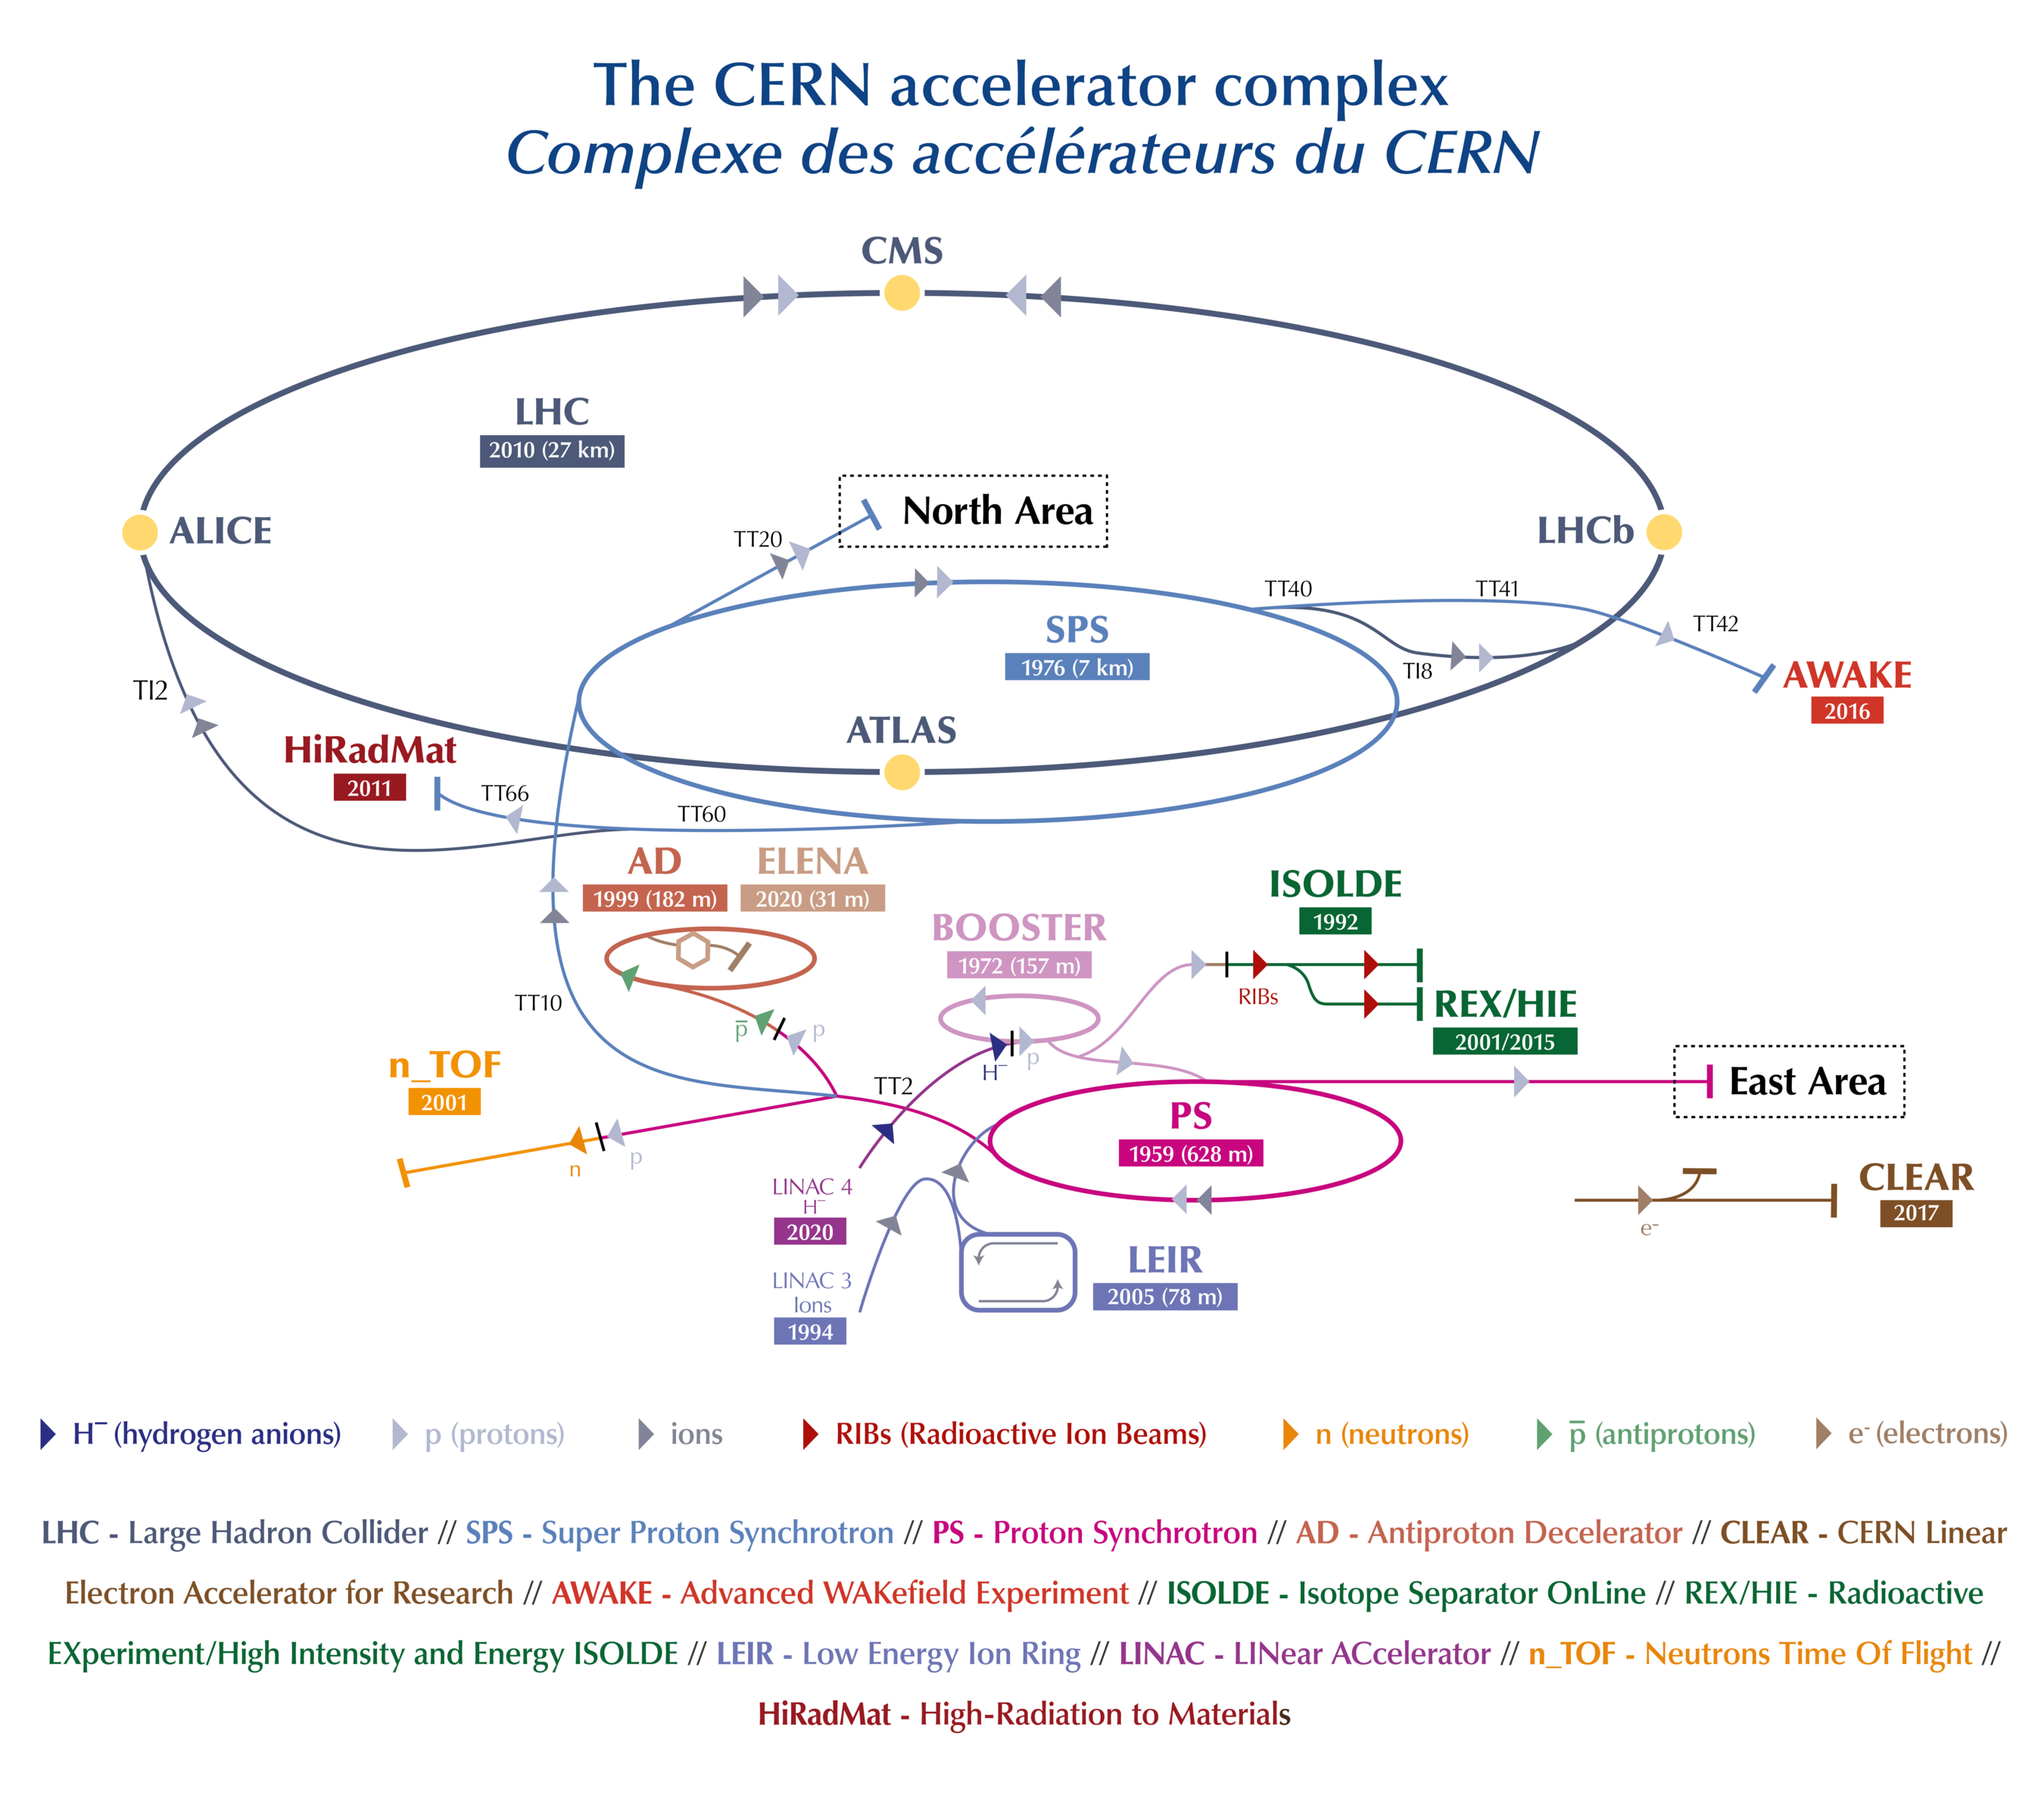
\includegraphics[width=0.98\textwidth]{figures/lhc-scheme.png}
  \caption[A schematic of the CERN accelerator complex]%
  {A schematic of the CERN accelerator complex~\cite{image-lhc-scheme}}%
  \label{fig:lhc}
\end{figure}

\subsection{
  Integrated Luminosity
}\label{ch_cms:cms-lumi}

The number of events generated in a collisions for a given process is
\begin{equation}
  N = L \sigma
\end{equation}
where \(\sigma \) is cross-section of the process
and \(L\) is the luminosity of the \gls{LHC}.

\begin{figure}[!ht]
  \centering
  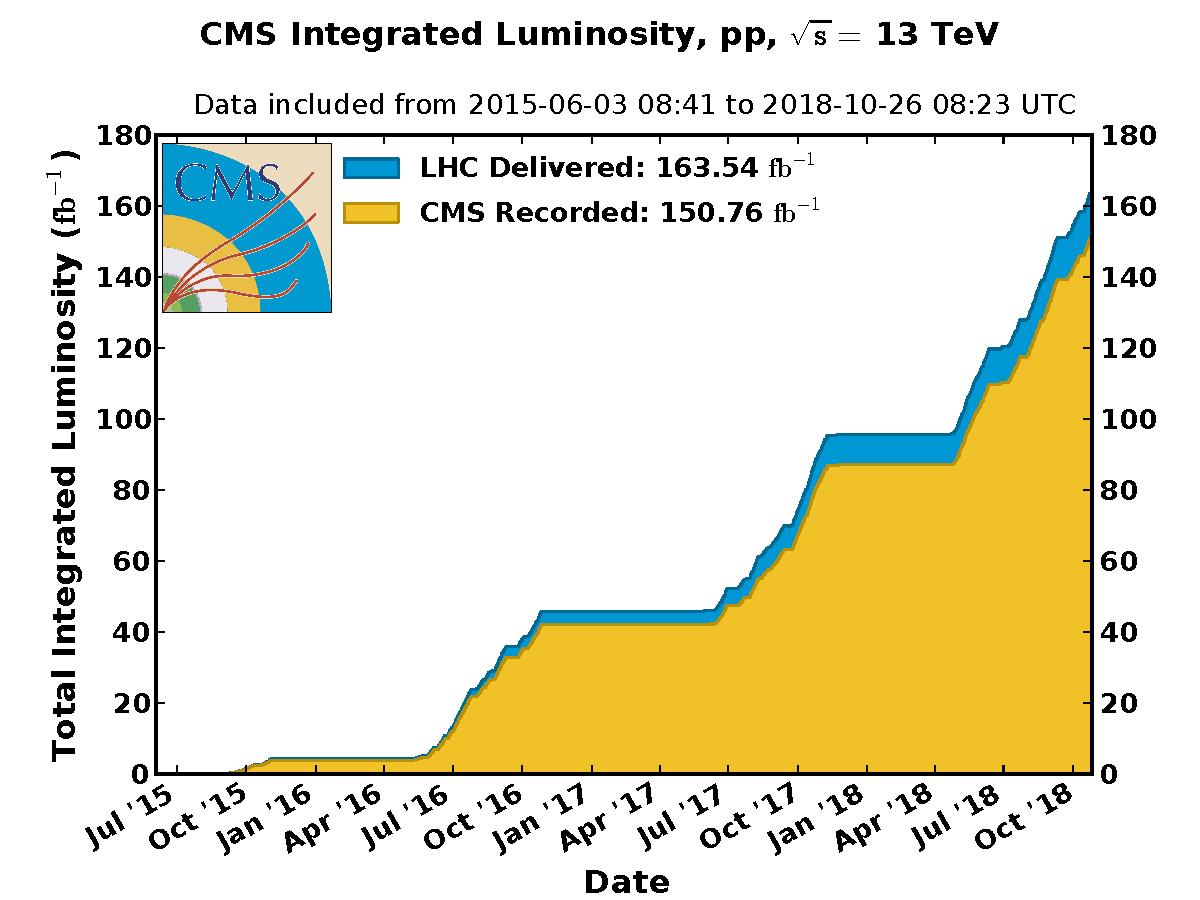
\includegraphics[width=0.5\textwidth]{figures/int_lumi_pp_run2.pdf}
  \caption[Cumulative delivered and recorded luminosity versus
    time for 2015--2018 proton-proton collisions]%
  {Cumulative delivered and recorded luminosity versus
    time for 2015--2018 proton-proton collisions~\cite{plot-cms-lumi}}%
  \label{fig:int-lumi}
\end{figure}

Cumulative luminosity delivered and recorded by \gls{CMS} during run-2 operation
in shown in Figure~\ref{fig:int-lumi}.
For run-2 standard physics analysis luminosity recorded during
2016--2018 is considered, and only runs certified as ``golden'' by \gls{CMS}
Luminosity \gls{POG} for analysis are used. The total luminosity for run-2
standard physics is 137.19\fbinv{}
and separately for years in Table~\ref{tab:years-lumi}
~\cite{CMS-PAS-LUM-17-001,CMS-PAS-LUM-17-004,CMS-PAS-LUM-18-002}.

\begin{table}[!ht]
  \centering
  \caption[Standard physics luminosity for run-2]%
  {Standard physics luminosity for run-2}
  \begin{tabular}{cccc}
    \toprule
    2016          & 2017          & 2018          & run-2          \\ \midrule
    35.92\fbinv{} & 41.53\fbinv{} & 59.74\fbinv{} & 137.19\fbinv{} \\
    \bottomrule
  \end{tabular}%
  \label{tab:years-lumi}
\end{table}

\section{
  The CMS Detector
 }\label{ch_cms:cms}

The \gls{CMS} detector is a general purpose detector.
A cutaway view of the detector is shown in Figure~\ref{fig:cms-cutaway}.
It is cylindrical detector 21\m{} long, 15\m{} in diameter,
and weighs about 14000 tonnes.
The detector is built in slices with central region called ``barrel'',
and two ``endcap'' regions.
A superconducting solenoid generated magnetic field of 3.8\Tesla{} inside
and 2\Tesla{} outside to contain the magnetic field outside of solenoid
and support structure of the detector massive steel yokes are used.

\begin{figure}[!ht]
  \centering
  \includegraphics[width=\textwidth]{figures/cms_cutway_ME4_2.pdf}
  \caption[The CMS detector cutaway view]%
  {The CMS detector cutaway view~\cite{image-cms-cutway}}%
  \label{fig:cms-cutaway}
\end{figure}

The slice view of \gls{CMS} in Figure~\ref{fig:cms-slice}
shows how different particles leave signature in \gls{CMS} detector.
Neutral particles such photons, neutrinos, and hadrons will leave no track
in \gls{ST}, and are identified by only energy deposited or missing energy.
Electrons are identified from the track in \gls{ST} and energy deposit
in \gls{ECAL}, hadrons are heavier and they pass through \gls{ECAL}
and deposit their energy completely in \gls{HCAL}, leaving only small fraction
of energy in \gls{ECAL}.
Since muons are \gls{MIP}, they pass through whole detector with very small
fraction of energy deposit in \gls{ECAL} and \gls{HCAL}.

\begin{figure}[!ht]
  \centering
  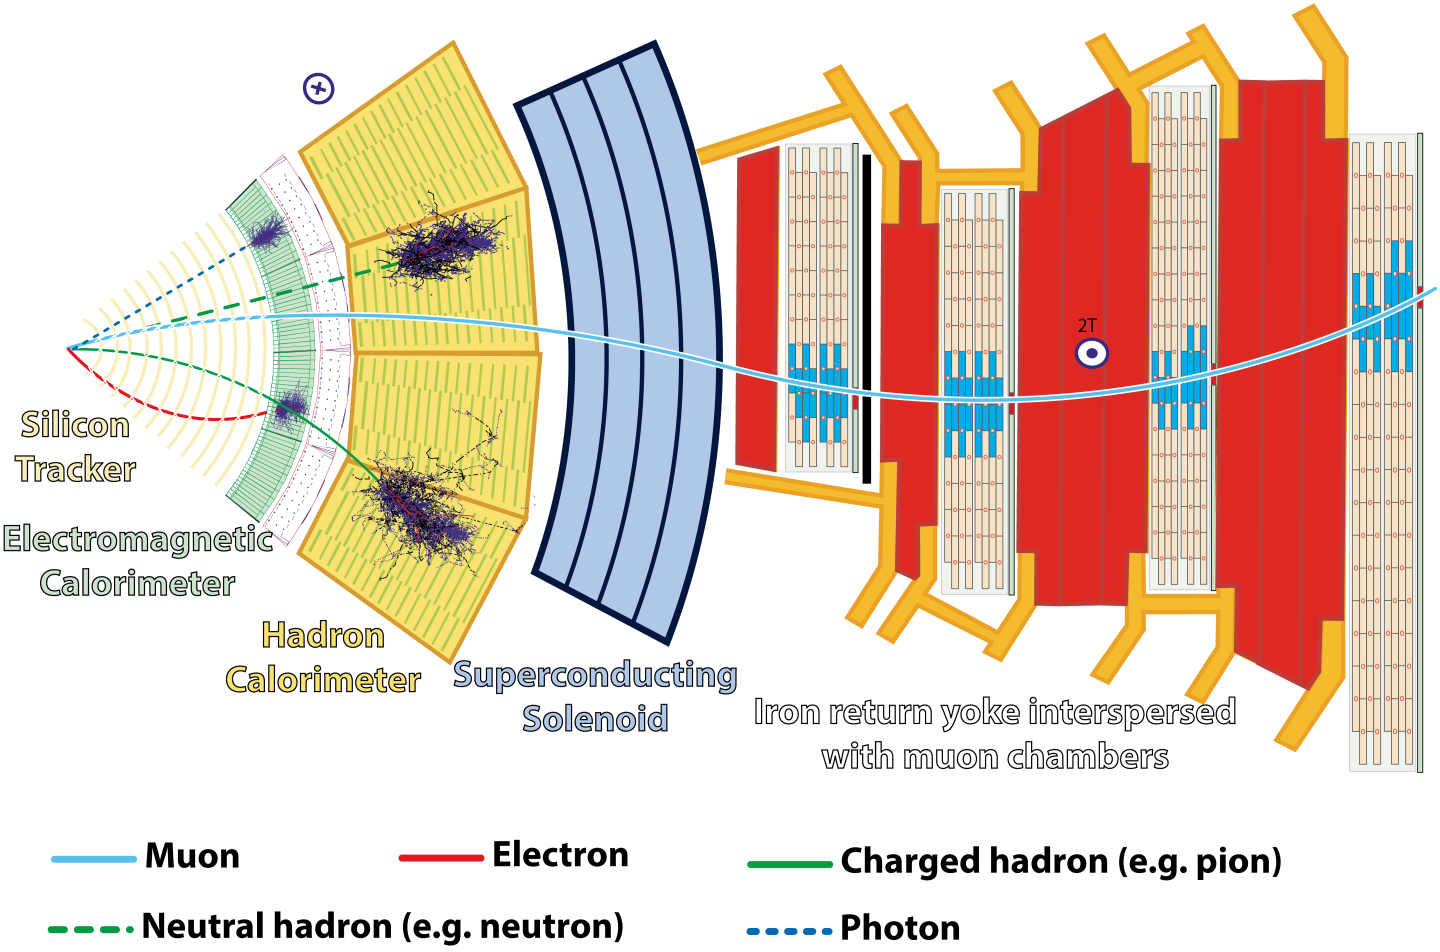
\includegraphics[width=\textwidth]{figures/cms_slice.png}
  \caption[The CMS detector slice view]%
  {The CMS detector slice view~\cite{image-cms-slice}}%
  \label{fig:cms-slice}
\end{figure}

\subsection{
  The CMS Coordinate System
}\label{ch_cms:cms-coordinate}

CMS uses \gls{IP} of collisions as origin to define right-handed
coordinate system. The \( z \)-axis is along the beamline,
the \( x \)-axis points toward the center of the \gls{LHC},
and the \( y \)-axis points upwards, toward Earth's surface.
The transverse plane \( x - y \) is used to calculate
transverse momentum \( p_{T} \) and energy \( E_{T} \).

To describe the direction of particles leaving the \gls{IP},
azimuthal \( \phi \) and polar \( \theta \) angles are used.
\( \phi \) is measured around the beam axis,
and \( \theta \) is measured from the beam axis.
In collider physics, pseudorapidity \( \eta \) (Lorentz invariant) is used
to describe direction from beam pipe instead of \( \theta \) as,

\begin{equation}
  \eta = - \ln[\tan{\theta/2}]
\end{equation}

and sometimes in terms of rapidity \( y \) as,

\begin{equation}
  y = \frac{1}{2} \ln{\frac{E+p_{z}}{E-p_{z}}}
\end{equation}

Particles kinematics can be completely described in terms of
\( p_{T} \), \( \eta \), \( \phi \), and \( E_{T} \) or mass.
The distance between the two particles \( \Delta R \) in \( \eta - \phi \) plane
is described as,

\begin{equation}
  \Delta R = \sqrt{ {(\Delta \eta)}^{2} + {(\Delta \phi)}^{2} }
\end{equation}



\subsection{
  The Superconducting Magnet
}

\subsection{
  The Tracking System
}

About \gls{CMS} Tracker System

Pixel Upgrade

\begin{figure}[!ht]
  \centering
  \begin{minipage}[c]{.62\textwidth}
    \includegraphics[trim={80pt 0 80pt 0},clip,width=\textwidth]%
    {figures/cms_pixel_phase1.pdf}
  \end{minipage}
  \begin{minipage}[c]{.35\textwidth}
    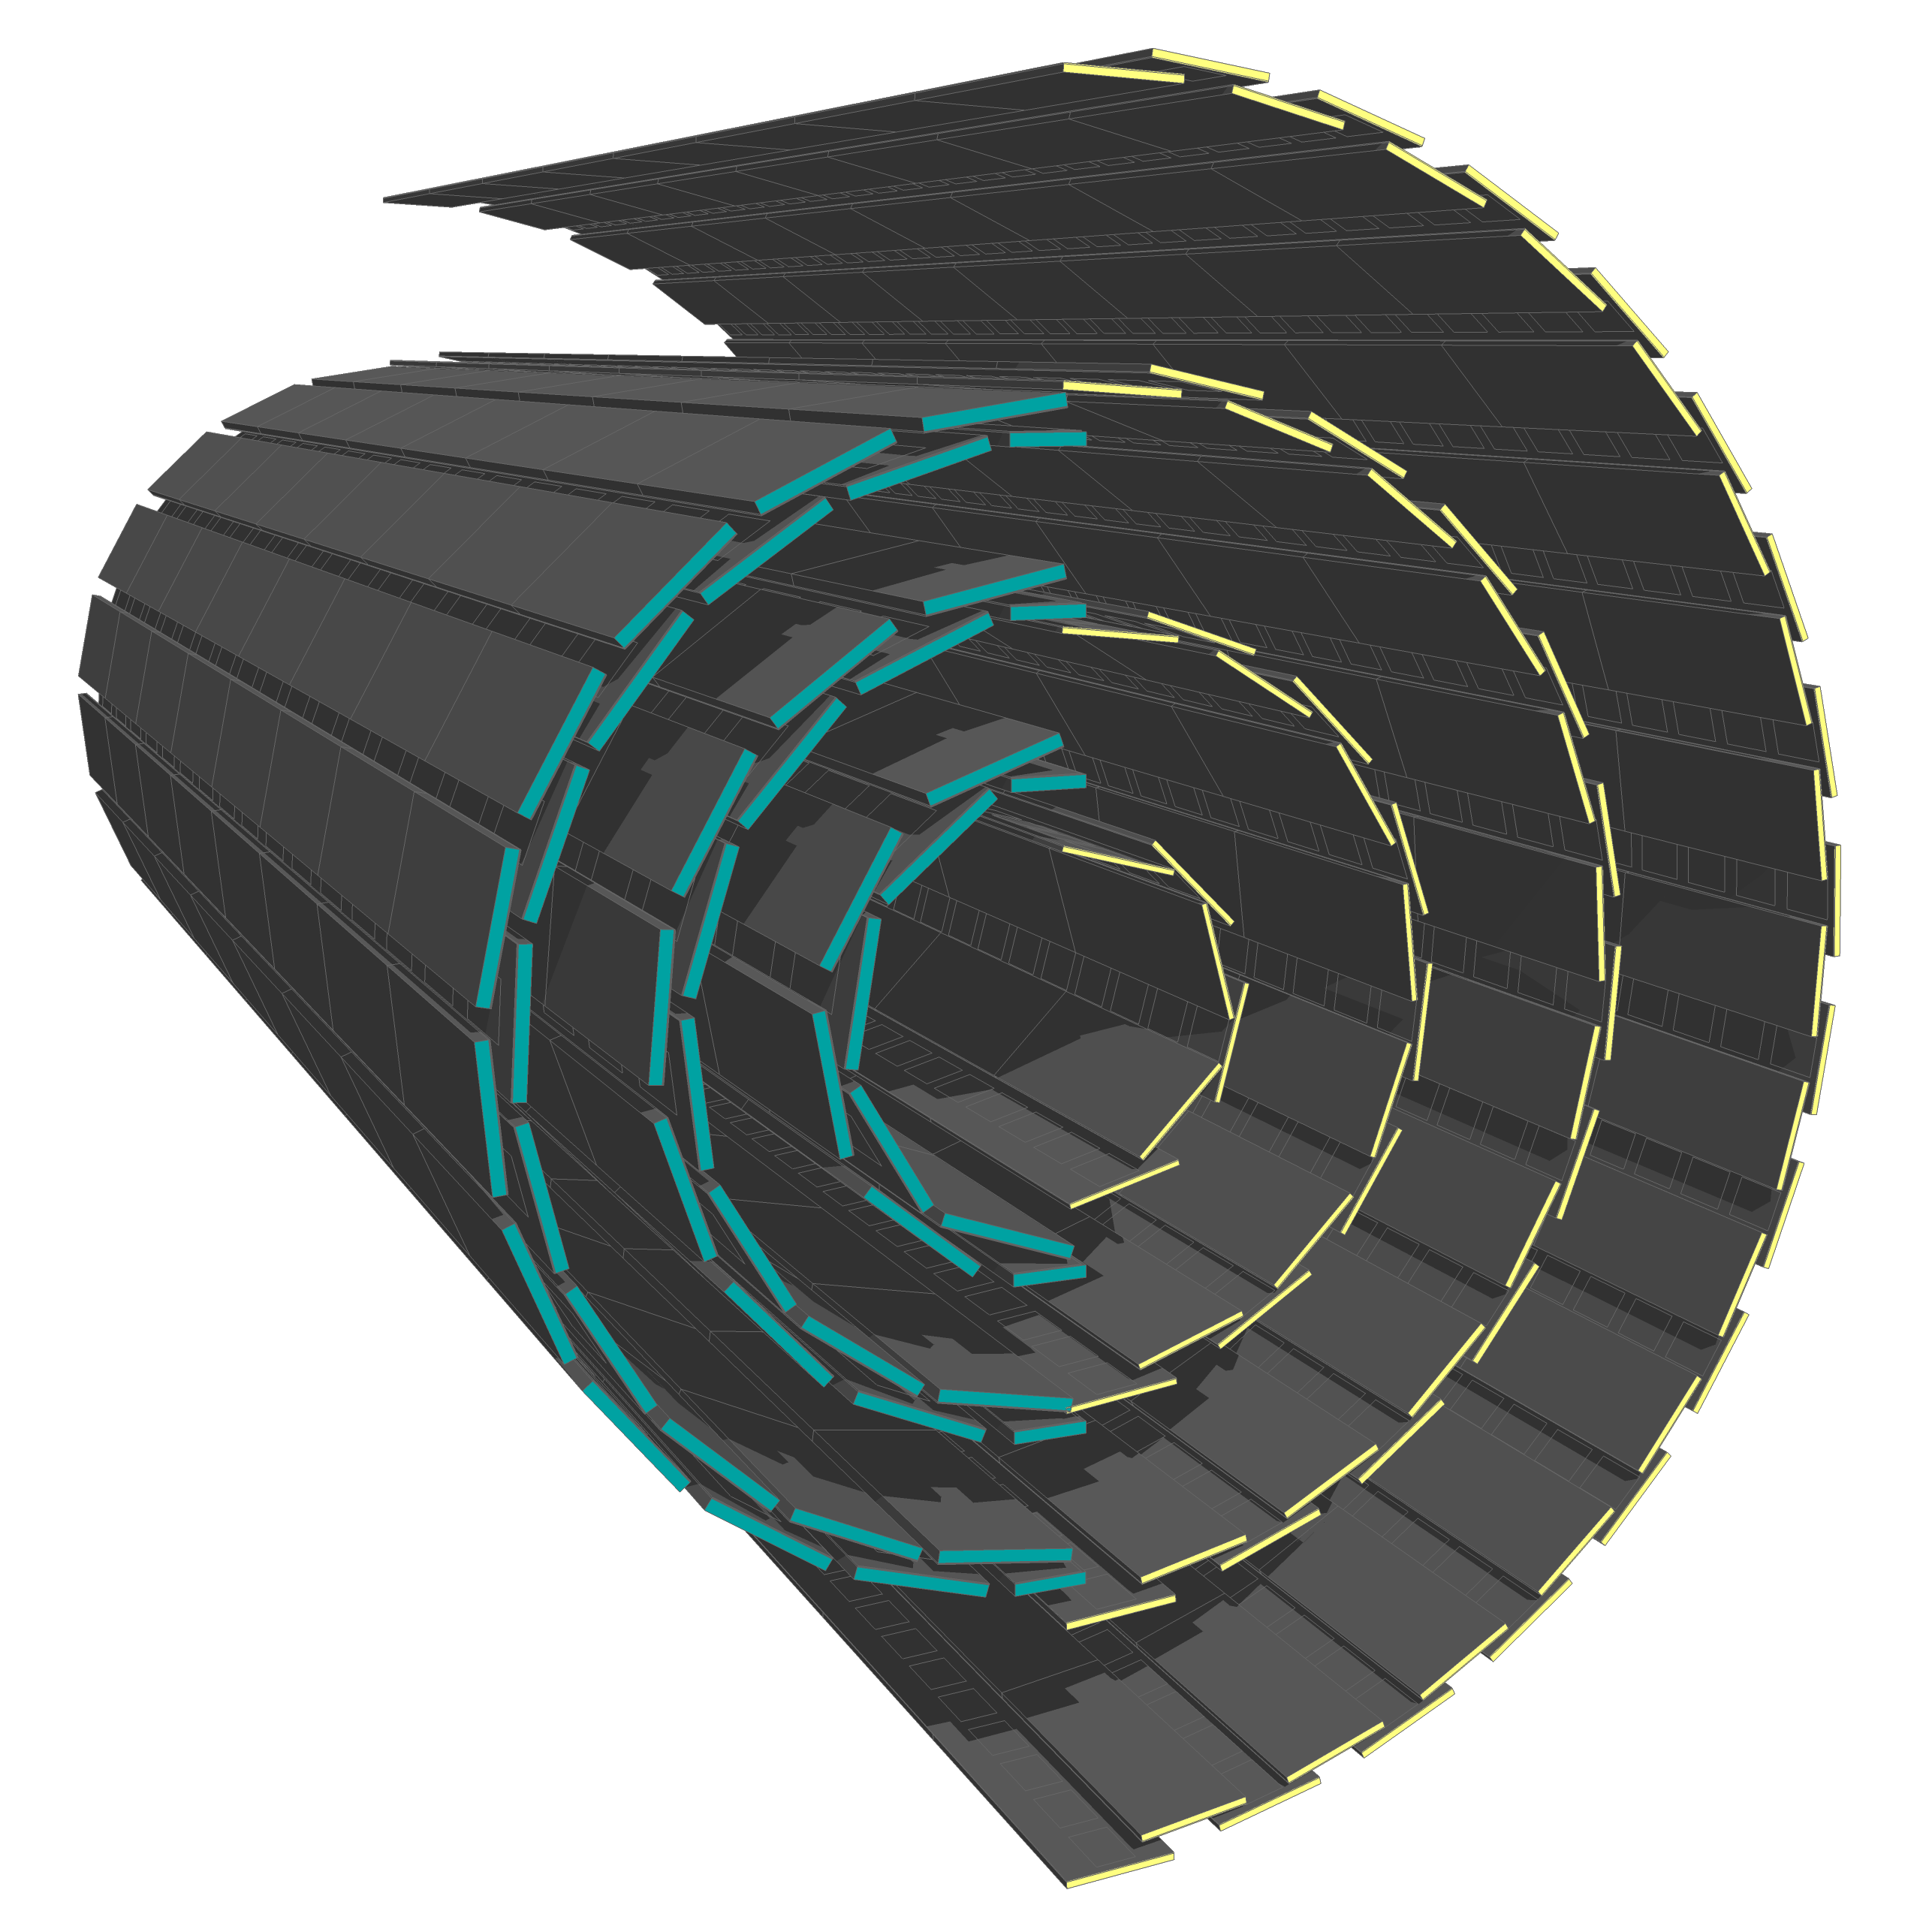
\includegraphics[width=\textwidth]{figures/cms_pixel_phase1_04.png}
  \end{minipage}
  \caption[The CMS pixel upgrade]%
  {The CMS pixel upgrade~\cite{image-cms-pixel}}%
  \label{fig:cms-pixel}
\end{figure}

\subsection{
  The Electromagnetic Calorimeter
}

\subsection{
  The Hadronic Calorimeter
}

\subsection{
  The Trigger System
}

\section{
  Endcap Calorimeter Upgrade
 }

About \gls{HGCAL} Upgrade
